\chapter{Analysing the properties of Data Models and Query Languages}\label{cha:datadef}


\epigraph{\textit{Therefore a science, the advancement of science, and the acquisition of science, is not simply the oblivion of old [scientifical] prejudices, or the fall of certain obstacles [to understanding], it is a new grid [of concepts] that masks certain things while allowing for the appearance of new knowledge}.}{--- Michel Foucault on \textit{The Chomsky-Foucault Debate: On Human Nature}, (1971)}


%\epigraph{\textit{The man who has no past, has no future: always remember that!}}{--- My grandfather about everything}

Before introducing graph based data models (Section \ref{sec:datamodelglit}), we  analyse the more widely adopted data models first. The reason for doing so is to check which are their weakest links, which are overcomed by our proposed data model (Chapter \vref{cha:graphsdef}). In particular, this chapter tackles structured (Section \vref{sec:relationalcmp}), nested relational and semistructured models (Section \vref{sec:semistructured}), and we'll analyse some ways to provide structured representations for unstructured data (fulltext, Section \vref{sec:unstructured}). For each data model we'll also briefly discuss their query languages.
\begin{figure}[!pth]
	%\begin{adjustbox}{max width=\textwidth}
	\begin{minipage}[b]{\textwidth}
		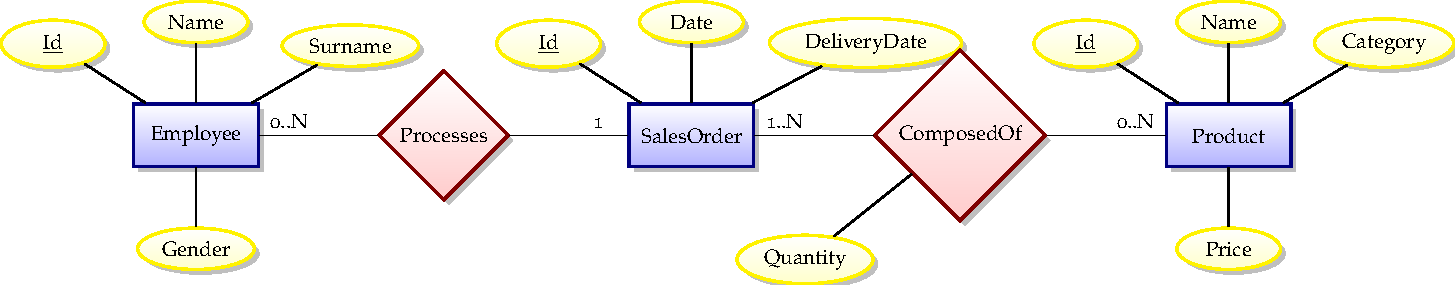
\includegraphics[scale=.6]{images/introduction/comparisons/relational/01erschema}
		\subcaption{Representing the ER model for a subset of a enterprise database, describing that each employee is able to create sales order formed by at least one product. }
		\label{fig:erschema}
	\end{minipage}\quad

	\begin{minipage}[b]{\textwidth}
		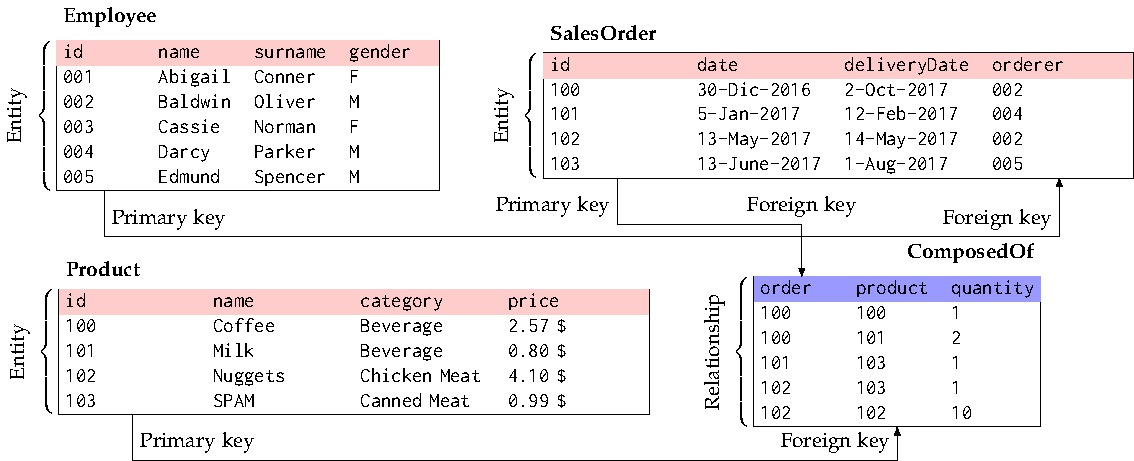
\includegraphics[scale=.7]{images/introduction/comparisons/relational/02instance}
		\subcaption{An instance of the overlying ER model. Please that some relations are directly expressed with Primary Key-Foreign Key relations (\textbf{Processes}), while others (\textbf{ComposedBy}) are require an intermediate table. The name of the relations appear on top of each table.}
		\label{fig:instance}
	\end{minipage}

	\begin{minipage}[b]{\textwidth}
		\centering
		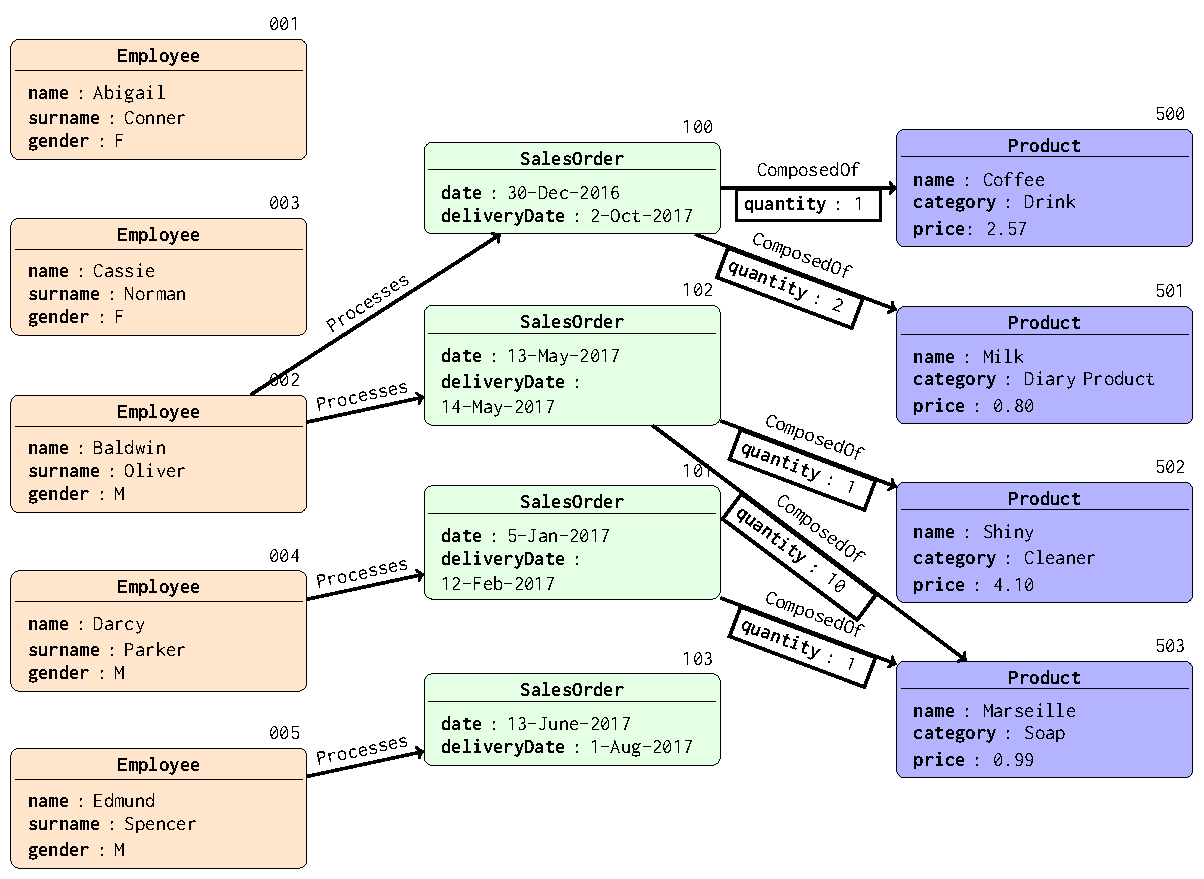
\includegraphics[scale=.6]{images/introduction/comparisons/relational/03dbasgraph}
		\subcaption{Representing the same relational database through a property graph. Please note that this is a faithful representation of the ER schema. The association between vertex and edge id's and their property-value association is described in Section \vref{sec:objid} (\textit{Object Identity})}
		\label{fig:graphofdb1}
	\end{minipage}
	%\end{adjustbox}
	\caption{While the process of modelling a relational database (\subref{fig:erschema}) requires to distinguish between entities and relationships, its instantiation in a logical database model discards them (\subref{fig:instance}). This information could be preserved within the property graph model (\subref{fig:graphofdb1}). }
	\label{fig:relationalinstance}
\end{figure}
